This event option is provided for the user to specify multiple existing
\href{http://peer.berkeley.edu}{PEER} ground
motion files.  For PEER events, the user is required to specify the
individual components for the EVENTS.  The \texttt{Add/Remove} buttons
at the top are to create and remove an event, as
per \Cref{subsec:multiple_existing}. For the PEER events, the user
specifies components acting in the individual degree-of-freedom
directions.  The \texttt{+} and \texttt{-} buttons add and remove
components with remove removing all components selected. Each
component in a PEER event can have their own scale factor, again a
number or a random variable.

\begin{figure}[!htbp]
  \centering {
    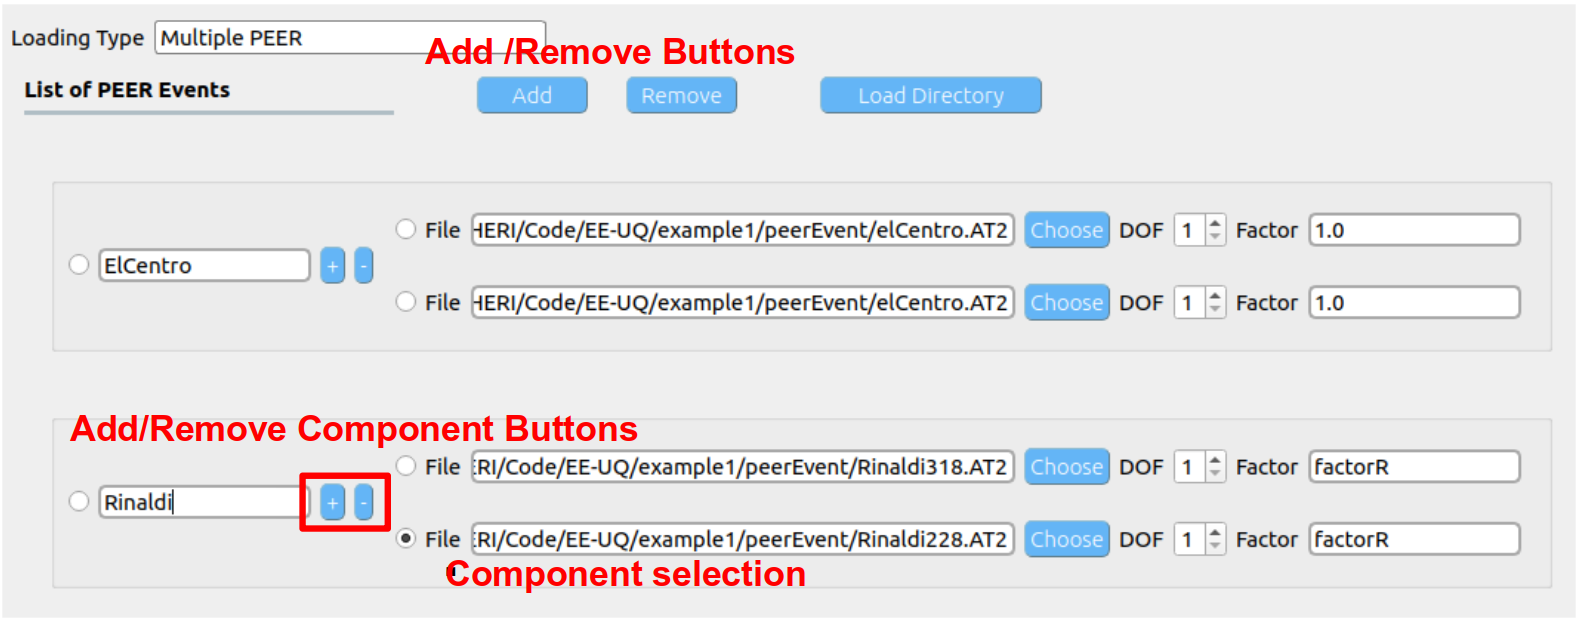
\includegraphics[width=0.8\textwidth]
    {usage/figures/multiplePEER.png} }
  \caption{\texttt{Multiple PEER} loading type}
  \label{fig:figure6}
\end{figure}

If the user has multiple events to load, they can again place all the
PEER \texttt{.AT2} files into a separate folder and select
the \texttt{Load Directory} option. This will allow the user to select
a directory. Once selected, all \texttt{.AT2} files in that directory will be
loaded into the application. Similar to loading multiple SimCenter
events, should the user provide a file \texttt{Records.txt} in that
directory, the application will load all files in the list and set the
appropriate load factor. An example \texttt{Results.txt} file for multiple Peer
events is as shown below:

\begin{verbatim}
elCentro.AT2,1.5
Rinaldi228.AT2,2.0
Rinaldi318.AT2,2.0
\end{verbatim}

Random Variables: The user can, as mentioned, enter a string in the
factor field to specify that the factor is to be considered a random
variable. Subsequently, in the UQ panel the user must provide
information on the random variables distribution. Also, if multiple
events are specified, the event itself will be treated as a random
variable with each event being part of the discrete set of possible
events.
